\begin{task}{2, Common bifurcations in nonlinear systems}

The solution and plots for this tasks are produced in \verb|task2/non_linear_1_d.ipynb|. In addition, some specific plotting utilities are implemented in \verb|task2/ode_d_plotter.py|.

In this task we will compare these equations defining parameterized dynamical systems on $\mathbb{R}$.

System 1
$$\dot{x}_1(x) = \alpha - x^2$$

System 2
$$\dot{x}_2(x) = \alpha - 2x^2 - 3$$

We can get the equilibria for $\alpha - x^2$ by looking at the equation $$\alpha - x^2 = 0$$.
This equation has roots 
$$x = \pm \sqrt{\alpha}$$
so for $\alpha < 0$ there will be no equilibria at $\alpha = 0$ there will be one at $x = 0$ and for $\alpha > 0$ they will be $x = \pm \sqrt{\alpha}$.

For a set $\alpha$ an equilibrium $y$ is stable if $\dot x$ at the interval around it has the opposite sign as $x - y$.

Because $\alpha - x^2$ is a quadratic equation it has three intervals with different signs. It is negative at $$x \in (- \infty, -\sqrt{\alpha})$$
positive at $$x \in (-\sqrt{\alpha},\sqrt{\alpha})$$
and negative again at $$x \in (\sqrt{\alpha},\infty).$$

For the special case $\alpha = 0$ we can express the requirement as $-x^2 x < 0$ which does not hold for $x < 0$ so the equilibrium is unstable.

When looking at $\alpha > 0$ we see the following about the equilibria.

We write the requirement for $y = \sqrt{\alpha}$

$$\alpha - x^2 < 0 \land x - \sqrt{\alpha} > 0  \Leftrightarrow x > \sqrt{\alpha}$$
$$\alpha > x^2 \land x < \sqrt{\alpha} \Leftrightarrow x \in (-\sqrt{\alpha}, \sqrt{\alpha}).$$

From this we can see that the equilibrium at $x = \sqrt{\alpha}$ is next to two intervals for which the requirement holds $$x > \sqrt{\alpha}$$ and $$x \in (-\sqrt{\alpha}, \sqrt{\alpha}).$$

We write the requirement for $y = -\sqrt{\alpha}$

$$\alpha < x^2 \land x > -\sqrt{\alpha} \Leftrightarrow x > \sqrt{\alpha}$$
$$\alpha > x^2 \land x < -\sqrt{\alpha} \Leftrightarrow \bot.$$

We can see that the equilibrium at $x = \sqrt{\alpha}$ is next to two intervals for which the requirement does not hold 
$$x \in (-\sqrt{\alpha}, \sqrt{\alpha})$$ 
and $$x < -\sqrt{\alpha}.$$

From these we can construct the bifurcation diagram by plotting the functions $\sqrt{\alpha}$ and $-\sqrt{\alpha}$.

The first parameterized system undergoes a saddle-node bifurcation at $\alpha = 0$ this is obvious from the telltale fork in the diagram in part a of the Figure \ref{fig:forks} and of course from the fact that the equation is the normal form of the saddle-node bifurcation.

To construct example trajectories we use points that are in intervals of different signs for both polynomials at both values of $\alpha$. We then calculate the endpoint of the trajectory after simulating using \verb|scipy.integrate.solve_ivp| and draw an arrow from the starting point to the endpoint. This is valid because if the value diverges the arrow will point towards the divergence and if it converges it will point towards the convergence, a stable orbit is impossible in the given systems.

$$\alpha = 1$$

\begin{figure}[H]
    \centering
    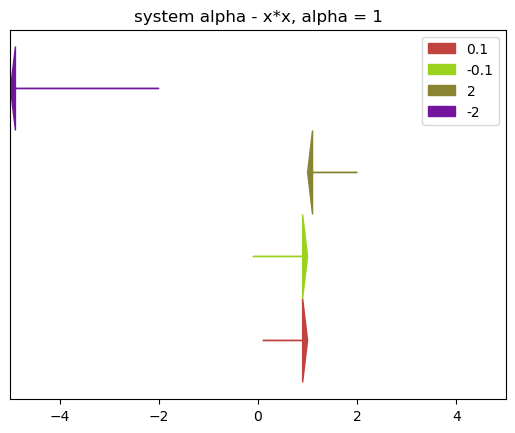
\includegraphics[width=0.45\textwidth]{images/1+1.png}
    \caption{System 1 at $\alpha = 1$ the color indicates the starting coordinate in $\mathbb{R}$ (see legend).}
    \label{fig:1+1}
\end{figure}

\begin{figure}[H]
    \centering
    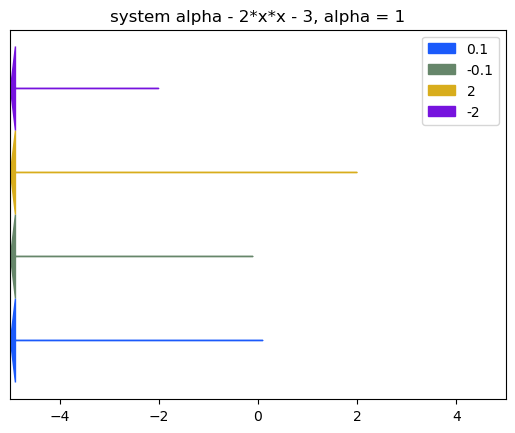
\includegraphics[width=0.45\textwidth]{images/2+1.png}
    \caption{System 2 at $\alpha = 1$ the color indicates the starting coordinate in $\mathbb{R}$ (see legend).}
    \label{fig:2+1}
\end{figure}

and therefore System 1 at $\alpha = 1$ has stable states

$$1 - x^2 = 0$$ 
$$x = 1 , x = -1$$

$$1 - 2x^2 - 3 = 0 $$ 
$$2x^2 = -2$$

has no real solutions and therefore System 1 at $\alpha = 1$ has stable states has no stable states

Any homeomorfism proving topologically equivalence is required to map orbits of one system onto orbits of another system. System 1 at $\alpha = 1$ and System 2 at $\alpha = 1$ are therefore not topologically equivalent because there is no way to map an empty set of orbits onto a non empty set or vice versa.

$$\alpha = -1$$

\begin{figure}[H]
    \centering
    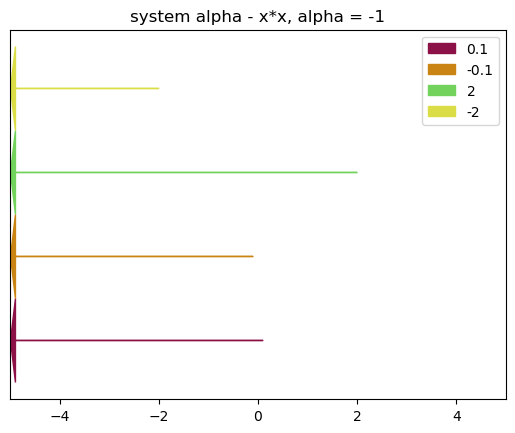
\includegraphics[width=0.45\textwidth]{images/1-1.png}
    \caption{System 1 at $\alpha = -1$ the color indicates the starting coordinate in $\mathbb{R}$ (see legend).}
    \label{fig:1-1}
\end{figure}

\begin{figure}[H]
    \centering
    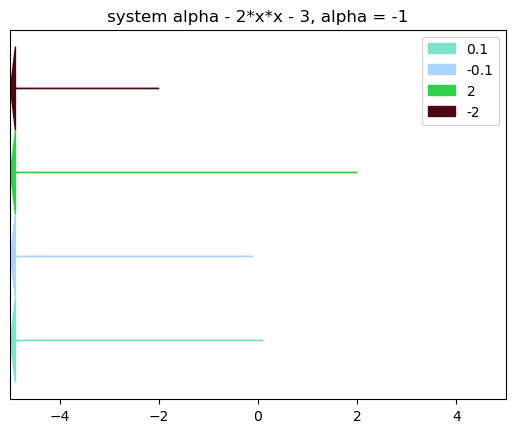
\includegraphics[width=0.45\textwidth]{images/2-1.png}
    \caption{System 2 at $\alpha = -1$ the color indicates the starting coordinate in $\mathbb{R}$ (see legend).}
    \label{fig:2-1}
\end{figure}

The polynomial
$$- 1 - x^2 = 0$$
has no real solution 
$$x^2 = -1$$
and therefore System 1 at $\alpha = -1$ has no stable points.

The polynomial
$$-1 -2x^2 - 3 = 0$$
$$2x^2 = -4$$
has no real solutions
and therefore System 2 at $\alpha = -1$ has no stable points.

System 1 at $\alpha = -1$ and System 2 at $\alpha = -1$ are topologically equivalent because if we take the identity mapping on $\mathbb{R}$ this mapping is bijective and continuous (it's inverse is equal to it and therefore also continuous) and it maps the empty set of orbits of System 1 at $\alpha = -1$ onto the empty set of orbits of System 2 at $\alpha = -1$.

Looking at figures in \ref{fig:forks} we can see that both systems undergo one bifurcation. We can also see that before then the systems have no stable points. Afterwards they have one stable and one unstable point, these are the defining characteristics of the one-dimensional saddle-node bifurcation. This is an argument as to why these parametrized systems have the same normal form as all parametrized systems that undergo the same bifurcations have the same normal form.

\begin{figure}[H]
    \centering
    \subfigure[System 1]{
    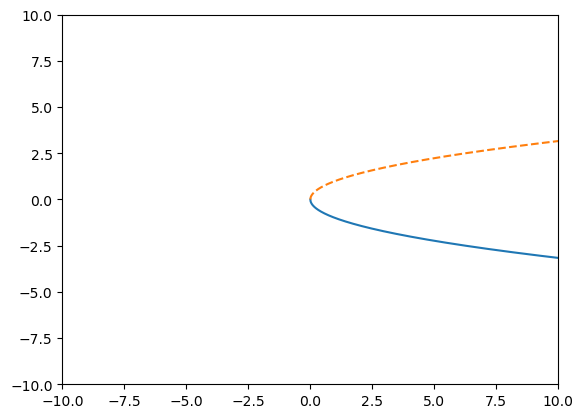
\includegraphics[width=0.45\textwidth]{images/bifurcationdiagram1.png}}
    \subfigure[System 2]{
    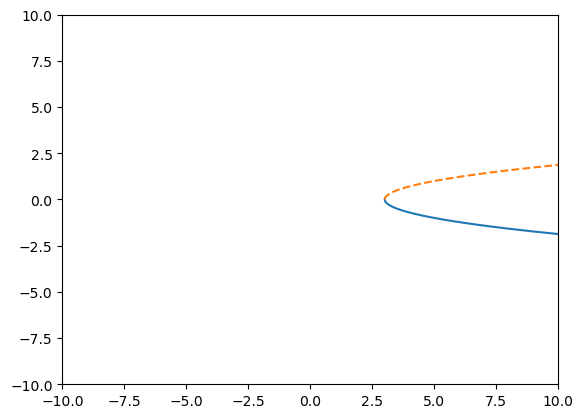
\includegraphics[width=0.45\textwidth]{images/bifurcationdiagram2.png}}
    \caption{The x coordinate indicates the $\alpha$, the y coordinate of the dotted curves indicates the coordinate in $\mathbb{R}$ of the stable equilibrium and the y coordinate of the full curves indicates the coordinate in $\mathbb{R}$ of the unstable equilibrium}
    \label{fig:forks}
\end{figure}

\end{task}